\lhead{Lecture 1: 10 October 2019}
\chapter{Introducing Differential Geometry}%

Structure: will do only differential geometry (maths methods) in the first 12 lectures, first 4 weeks. Afterwards the connection to the physics will be made.
We will develop a mathematical language that allows us to write valid equations involving vectors, similar to dimensional analysis for physicists. The physics will be introduced with the action principle.

Extra book: ``Geometry, Topology, and Physics'' by Nakahara.

Office Hours: Friday $4 \rightarrow 5$ in B2.13

Extra stuff not examinable. Lectures are what matters.

\section{Manifolds}%
\label{sec:manifolds}

\begin{definition}[]
An \emph{$n$-dimensional manifold} $\mathcal{M}$ is a space that locally looks like $\mathbb{R}^n$.
More precisely, we require
\begin{enumerate}
  \item For each point $p \in \mathcal{M}$, there is a map $\phi \colon \mathcal{O} \to U$ where $\mathcal{O} \subset \mathcal{M}$ is an open set with $p \in \mathcal{O}$ and $U \subset \mathbb{R}^n$.
    We will think of $\phi(p) = (x^1(p), \dots, x^n(p))$ as coordinates on $\mathcal{O} \subset \mathcal{M}$.

    This map must be a \emph{homeomorphism}:
    \begin{enumerate}
      \item injective (or 1-1) $p \neq q \implies \phi(p) \neq \phi(q)$
      \item surjective (or onto) $\phi(\mathcal{O}) = U$\par
	These ensure that $\phi^{-1}$ exists.
      \item both $\phi$ and $\phi^{-1}$ are continuous
    \end{enumerate}
  \item If $\mathcal{O}_\alpha$ and $\mathcal{O}_\beta$ are two open sets with 
    \begin{equation}
      \phi_\alpha: \mathcal{O}_\alpha \to U_\alpha \text{ and } \phi_\beta: \mathcal{O}_\beta \to U_\beta
    \end{equation}
    then the \emph{transition functions} $\phi_\alpha \circ \phi^{-1}_\beta: \phi_\beta(\mathcal{O}_\alpha \cap \mathcal{O}_{\beta}) \to \phi_\alpha (\mathcal{O}_\alpha \cap \mathcal{O}_\beta)$ are smooth (ie.~infinitely differentiable).
    The $\phi_\alpha$ are called \emph{charts}. The idea is that there may be different ways to assign coordinates to a given point $p \in \mathcal{M}$.
    The collection of all charts is called an \emph{atlas}.
    We require that these coordinate systems are mutually compatible. This is depicted in Figure \ref{fig:manifold}.
\end{enumerate}
\end{definition}

% F1
\begin{figure}[tbhp]
  \centering
  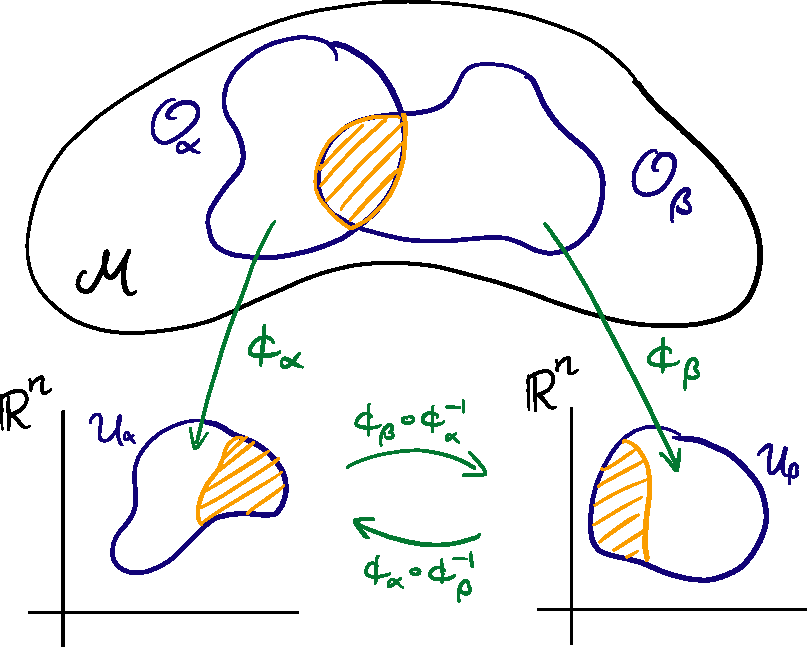
\includegraphics[width=0.5\linewidth]{lectures/F1.pdf}
  \caption{An illustration of charts on a manifold}
  \label{fig:manifold}
\end{figure}

\begin{example}[$\mathbb{R}^n$]
  $\mathbb{R}^n$ or any open subset of $\mathbb{R}^n$ is a manifold. You only need a single chart.
\end{example}

\begin{example}[$S^1$]
  We can view this as $(\cos \theta, \sin \theta) \in \mathbb{R}^{2}$ with $\theta \in [0, 2\pi)$. The closed set $[0, 2\pi)$ means that we cannot differentiate at $0$. This is \underline{not} a good chart because it is not an open set. 
  We need at least two charts, depicted in \ref{fig:L1F2}:
  \begin{equation}
    \begin{alignedat}{2}
      \phi_1 \colon \mathcal{O}_1 &\to (0, 2\pi)  \qquad&\qquad
      \phi_2 \colon \mathcal{O}_2 &\to (-\pi, \pi) \\
      p &\mapsto \theta_1 &
      p &\mapsto \theta_2
    \end{alignedat}
  \end{equation}
  The transition function is 
  \begin{equation}
    \theta_2 = \phi_2(\phi_1^{-1}(\theta_1)) = 
    \begin{cases}
      \theta_1, & \theta_1 \in (0, \pi) \\
      \theta_1 - 2\pi, & \theta_1 \in (\pi, 2\pi)
    \end{cases}
  \end{equation}
\begin{leftbar}
  \begin{remark}
    The fact that the coordinates go bad in the case of closed sets, similar to spherical polar coordinates, does not bother us too much for physical applications.
  \end{remark}
\end{leftbar}
\end{example}
\begin{figure}[htpb]
  \centering
  \def\svgwidth{0.7\columnwidth}
  \input{lectures/F2.pdf_tex}
  \caption{The two charts $\phi_1, \phi_2$ form an atlas of the manifold $S^1$.}
  \label{fig:L1F2}
\end{figure}

Since we can map $\mathcal{M} \to \mathbb{R}^n$ (at least locally), anything we can do on $\mathbb{R}^n$, we can now also do on $\mathcal{M}$ (e.g.~differentiation).

\begin{leftbar}
  \begin{remark}
    Note that at the moment, the distance in $\mathbb{R}^n$ cannot be translated back to the manifold. This is because the maps $\phi_\alpha$ are arbitrary.
  \end{remark}
\end{leftbar}

\begin{definition}[Diffeomorphism]
  A \emph{diffeomorphism} is a smooth homeomorphism $f: \mathcal{M} \to \mathcal{N}$ between two manifolds.
  I.e.~two manifolds are diffeomorphic if the map $\psi \circ f \circ \phi^{-1}: U \to V$ is smooth for \underline{all} charts $\phi: \mathcal{M} \to U \subset \mathbb{R}^n$ and $\psi: N \to V \subset \mathbb{R}^n$.
\end{definition}

\begin{leftbar}
  \begin{remark}
    There are interesting properties of $S^7$ and $\mathbb{R}^{4}$. You can find two atlasses of these manifolds such that the two atlasses are not diffeomorphic to each other.
    These are called \emph{exotic} manifolds; they are homeomorphic but not diffeomorphic to their respective Euclidean counterparts.
    As far as we know, there is yet no application of this in physics.
  \end{remark}
\end{leftbar}

\begin{leftbar}
  \begin{remark}
    These manifolds have intrinsic meaning and do not depend on an embedding. Physically, the $3+1$-dimensional spacetime is a manifold that we do not think is embedded in any higher dimensional space.
  \end{remark}
\end{leftbar}




